\chapter{Proposta da plataforma}
Esse projeto propõe o desenvolvimento de uma plataforma com o objetivo de auxiliar o aprendizado de novo vocabulário. Existem múltiplas aplicações com o mesmo fim no mercado atualmente, cada uma delas com suas particularidades, a seguir tem-se uma breve descrição de alguns exemplos:

\section{Aplicações Semelhantes}

\subsection{Duolingo}
Duolingo é uma plataforma que contém um aplicativo \textit{mobile} e um sistema web para o aprendizado de línguas estrangeiras utilizando repetição espaçada. A plataforma utiliza-se de conceitos de gamificação para manter o usuário engajado na plataforma. O usuário progride através de de uma árvore de desafios e a dificuldade das sentenças a serem aprendidas aumentam gradualmente. Não é possível criar \textit{flashcards} customizados e dessa forma o usuário fica limitado ao vocabulário que é escolhido pelo Duolingo para o aprendizado da linguagem.

\begin{figure}[H]
\caption{\label{fig:duolingo}Duolingo}
\begin{center}
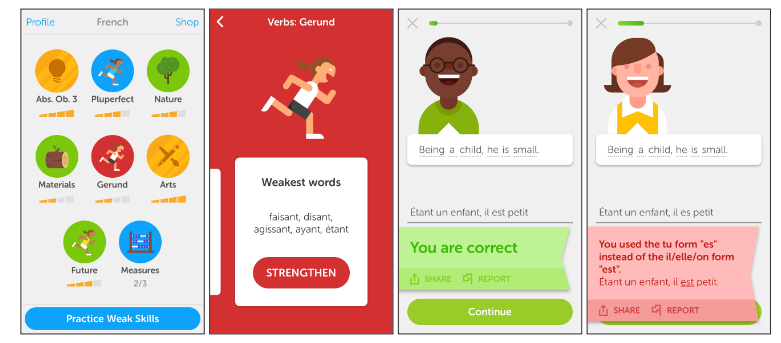
\includegraphics[scale=0.60]{duolingo}
\end{center}
\legend{Fonte: A Trainable Spaced Repetition Model for Language Learning, 2016}
\end{figure}

O algoritmo utilizado para repetição espaçada no aplicativo é chamado de HLR ou \textit{Half-Life Regression} que utiliza conceitos do método de Leitner juntamente com idéias do método de Pimsleur através de aprendizado de máquina para calcular os intervalos de estudo (SETTLES et al., 2016).

\subsection{Super Memo}
Super Memo é um método de aprendizagem e também um \textit{software} desenvolvido primariamente por Piotr Woźniak, um pesquisador que publicou vários artigos na área de repetição espaçada e aprendizado. O software permite que o usuário selecione pacotes de \textit{flashcards} já criados para sessões de estudo ou criar seus próprios \textit{flashcards} para estudar. É utilizado uma versão proprietária do algoritmo SM que foi descrito no Capítulo 2 para calcular os intervalos de estudo.

\begin{figure}[H]
	\caption{\label{fig:supermemo}Super Memo}
	\begin{center}
		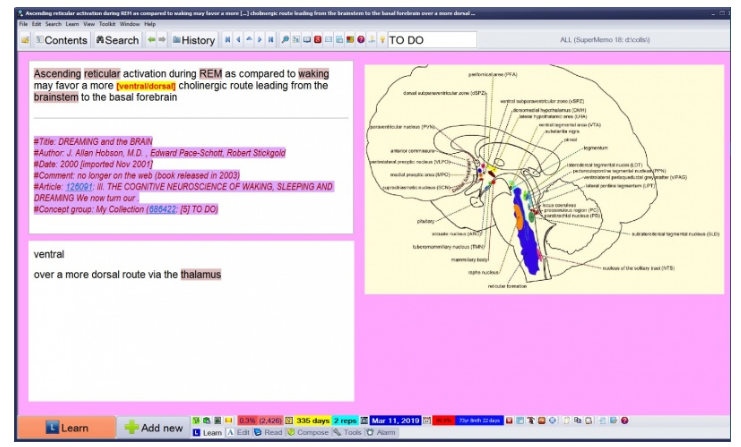
\includegraphics[scale=0.60]{supermemo}
	\end{center}
	\legend{Fonte: Disponível em: https://help.supermemo.org/wiki/SuperMemo\_Screenshot\_Tour. Acesso em: 01 out. 2019.}
\end{figure}

\subsection{Anki}
Anki é um software para memorização de conteúdo, não apenas vocabulário ou material relacionado a línguas estrangeiras mas qualquer conteúdo que envolva memorização. Funciona de forma semelhante ao Super Memo. Permite que o usuário use pacotes de \textit{flashcards} ou crie seus próprios \textit{flashcards}. O algoritmo de aprendizado espaçado utilizado por Anki é a versão 2.0 do algoritmo SM ou também chamado de SM-2. A escolha da versão desse algoritmo de acordo com os desenvolvedores do Anki se deve ao fato que possui embasamento científico (ANKI, 2019) e também é código aberto, que permite a distribuição do Anki como \textit{software} livre e de código aberto para todos seus usuários.

\begin{figure}[H]
	\caption{\label{fig:anki}Anki}
	\begin{center}
		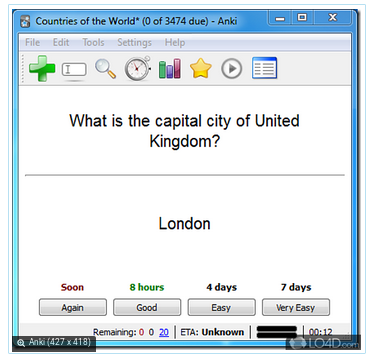
\includegraphics[scale=0.60]{anki}
	\end{center}
	\legend{Fonte: Disponível em: https://anki.en.lo4d.com/screenshots. Acesso em: 01 out. 2019.}
\end{figure}


\section{Flashcard com leitura interativa}
A proposta desse projeto é criar uma plataforma que permita ao usuário aprimorar seu vocabulário através do método de repetição espaçada e \textit{flashcards} em conjunto com leitura de textos como artigos e notícias. Como foi descrito anteriormente no capítulo 3, o denominado aprendizado involuntário de novo vocabulário através um contexto textual é mais efetivo. A plataforma desenvolvida é composta de uma aplicação mobile para Android e iOS e um \textit{backend} para sincronizar dados entre as plataformas (mais detalhes sobre implementação no Capítulo 5). A escolha da plataforma \textit{mobile} deve-se ao fato de que a aplicação não requer nenhum \textit{input} complexo e a interface de \textit{touchscreen} é bastante intuitiva para o layout do aplicativo. Outro motivo que favoreceu a escolha da plataforma mobile é que o usuário pode praticar vocabulário mesmo não tendo acesso a um computador, sendo assim possível utilizar o aplicativo fora de casa ou no transporte público. No aplicativo o usuário pode escolher a partir de uma lista de notícias uma que seja de seu interesse e na língua que está sendo estudada e a partir desse artigo ele pode selecionar as palavras que tiver dificuldade e diretamente ver a tradução dessas palavras, se desejado o usuário pode adicionar a palavra selecionada a uma lista de \textit{flashcards} para estudar posteriormente. O usuário pode também criar listas de \textit{flashcards} customizados caso ele queira estudar palavras que não necessariamente pertencem a uma notícia fornecida pelo aplicativo. Como descrito anteriormente, o algoritmo de repetição espaçada escolhido para esse projeto foi o SM-2. Um dos motivos para a escolha desse algoritmo é o fato de ser bastante performático e pode rodar direto no dispositivo do usuário, outro motivo foi o fato de que o algoritmo possui código aberto e possui licença livre. Quando o usuário decidir revisar uma lista de \textit{flashcards}, o software calcula quais \textit{flashcards} devem ser mostrados e com qual frequência baseado na performance do usuário sem sessões anteriores. O aplicativo também mostrará notificações para o usuário lembrar-se de revisar os \textit{flashcards} quando for o melhor momento baseado na curva de esquecimento descrita no Capítulo 3.

